\addurlfn{capacitor-electron-plattform}{Capacitor-Community Electron Plattform}{https://github.com/capacitor-community/electron}
\addurlfn{electron-browserview}{Electron BrowserView}{https://electronjs.org/docs/latest/api/browser-view}

\subsection{Zielsetzung}

Das Hauptziel des Capacitor-BrowserView Plugins ist die Entwicklung eines Plugins für Capacitor, welches es Entwicklern ermöglicht, zusätzliche Webinhalte durch WebViews in Capacitor Anwendungen zu integrieren.
Das Plugin soll eine \ac{api} bereitstellen, mit der WebViews erstellt und gesteuert werden können.
Außerdem soll eine Kommunikation zwischen geladenen Webinhalten und der Anwendung ermöglicht werden.

\begin{figure}[H]
    \centering
    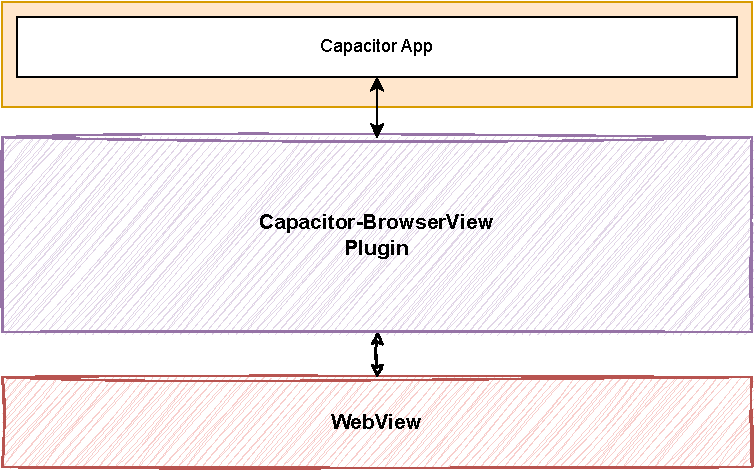
\includegraphics[width=\textwidth]{assets/03_Capacitor-BrowserView/01_Zielsetzung.drawio.pdf}
    \caption[Capacitor-BrowserView / Zielsetzung]{Zielsetzung des Capacitor-BrowserView Plugins}
\end{figure}

Als weiteres Ziel soll die Kompatibilität des Plugins mit der \fn{capacitor-electron-plattform} gewährleistet werden.
So soll das Plugin ohne zusätzlichen Aufwand sowohl in Mobile"=Anwendungen als auch in Desktop"=Anwendungen eingesetzt werden können.

Die vom Plugin implementierten WebViews werden auch als BrowserViews bezeichnet, um die Ähnlichkeit mit der \fn{electron-browserview} zu verdeutlichen.

\printfn
